\selectlanguage{english}%

\chapter{Fundamentos Fuzzy}
A lógica fuzzy, ou difusa, foi introduzida originalmente por Zadeh, em seu artigo "Fuzzy Sets" \cite{zadeh}. Sua teoria de conjunto diverge da booleana 
no tratamento dos valores lógicos das variáveis, podendo assumir qualquer valor entre 0 e 1. 

\section{Conjuntos Fuzzy}
\indent De acordo com a teoria de conjuntos clássica, um elemento $x$ qualquer, pode pertencer ou não à um conjunto universo de discurso $U$, $x \in U$. Chamando de $f_u(x)$ a função de pertinência de $x$ ao conjunto $U$. Desta forma, tem-se:

\begin{align}
	f_u(x) : U \rightarrow \{0,1\}
	&& f_u(x) =
	\begin{cases*}
		1 & se e somente se $x \in U$ \\
		0 & caso contrário
	\end{cases*}
	\label{eqFPertinencia}
\end{align}

Essa definição binária se encaixa bem em problemas restritos, cujo caráter dos sistemas reflita essa separação de estados, por exemplo a paridade ou não de uma das somas dos bits de uma mensagem binária. No entanto, grande parte dos sistemas estudados nas teorias de controle trabalha com grandezas que possuem limites não tão claros assim, como exemplo a temperatura. Apesar de ser matematicamente bem definida, existem descrições como "frio" e "quente" que não podem ser representadas com este conjunto binário, uma vez que são conceitos vagos e imprecisos. A abordagem fuzzy é capaz de tratar a pertinência nestes casos, de onde vem a origem de seu nome "difusa".

\section{Funções de Pertinência}
	\subsection{Variáveis Linguísticas}
	
	\begin{align}
		f_p(x) : U \rightarrow [0,1]
		\label{eqFuncPertFuzzy}
	\end{align}
	
	\begin{itemize}
		\item Clássica \\
		\item Triangular		
	\end{itemize}
	
	
\section{Inferência}

\subsection{Fuzzyficacão}

\subsection{Regras}
	
	\textbf{Regra i:}
	\begin{align}
		&\textbf{SE:} \text{ $v_1(t)$ é $M_{i1}$ e $v_2(t)$ é $M_{i2}$ e ... e $v_n(t)$ e $M_{in}$,} \\
		&\textbf{ENTÃO}: \ \ \begin{cases}
			\dot{x}(t) = A_ix(t) + B_iu(t),\\
			y(t) = C_ix(t)
		\end{cases}
	\label{eqRegraIGeral}
	\end{align}
	
	\textbf{Regra i:}
	\begin{align}
		\textbf{SE:}  \hspace{1cm} &\text{ $h_1(t)$ é $P_{1,i}$ e $h_2(t)$ é $P_{2,i}$,} \\
		\textbf{ENTÃO:} \hspace{1cm} & \dot{h}(t) =  A_i \Delta h_i(t) +  B_i \Delta u_i(t)
	\end{align}
	
	Cada regra definida implica um sistema linear diferente, que melhor representa a dinâmica da planta em cada região. Essas linearizações são baseadas nas variáveis de desvio, assim, para cada regra $i$, temos:
	\begin{align}
		\Delta h_i(t) =
		\begin{bmatrix}
			h_1(t) - \bar{h_{1i}} \\
			h_2(t) - \bar{h_{2i}} \\
			h_3(t) - \bar{h_{3i}} \\
			h_4(t) - \bar{h_{4i}}
		\end{bmatrix} 
		&&
		\Delta u_i(t) = 
		\begin{bmatrix}
			u_1(t) - \bar{u_{1i}} \\
			u_2(t) - \bar{u_{12}}
		\end{bmatrix}
	\end{align}	

\section{Modelo Fuzzy Takagi-Sugeno}
	\begin{equation}
	\begin{aligned}
		w_{1}(t) = M_1(h_1(t)) * N_1(h_2(t)) \\
		w_{2}(t) = M_1(h_1(t)) * N_2(h_2(t)) \\
		w_{3}(t) = M_2(h_1(t)) * N_1(h_2(t)) \\
		w_{4}(t) = M_2(h_1(t)) * N_2(h_2(t))
	\end{aligned}
	\end{equation}
	
	\begin{align}
		\dot{h}(t) = \frac{\sum_{i=1}^{4}  w_i(h(t))(A_i \Delta h_i(t) +  B_i \Delta u_i(t))}{\sum_{i=1}^{4} w_i(h)}
	\end{align}

\indent A Teoria Fuzzy tem seu princípio cunhado por \cite{zadeh65}. Os trabalhos seguintes, como o \cite{takagi_sugeno} abordaram sua utilização para a modelagem de sistemas complexos por meio de aproximações, utilizando uma teoria de conjuntos diferente da convencional.

\subsection{Conjuntos Fuzzy}
\indent A teoria de conjuntos convencional utiliza lógica booleana para definir os valores lógicos das funções de pertinências dos conjuntos. Assim, dado $X$ o universo de discurso de um determinado conjunto $C$, um elemento genérico $x$ tem sua função de pertinência ao conjunto $C$ dado por:

\begin{align*}
f_{C}(x)&:X \rightarrow \{0,1\} \quad \\
f_{C}(x)&= 
\begin{cases}
1 \text{ se e somente se x} \in C \\
0 \text{ se e somente se x} \notin C\\
\end{cases}
\end{align*}

Existem, no entanto, situações em que a definição dos conjuntos de seus limites se tornam muito subjetivos. Nestas situações, a utilização da lógica difusa apresenta vantagens para a modelagem de sistemas. 

Considere-se como exemplo a temperatura de uma sala. Pode-se definir dois conjuntos de estados \{quente,frio\}. No entanto, torna-se um pouco confuso e arbitrário decidir em qual destes conjuntos um estado específico se encaixa. Utilizando funções de pertinências não binárias, observa-se o \textbf{quanto} determinada temperatura se encaixa em cada um dos conjuntos. Funções de pertinências fuzzy são definidas da forma:

\begin{align*}
f_{C}(x)&:X \rightarrow [0,1]
\end{align*}

\subsection{Funções De Pertinência}
Existem várias normas e regras disponíveis para funções de pertinência. Este trabalho considera a norma triangular. Seguindo o exemplo dado, dada uma temperatura $x$ verifica-se o quão pertencente aos conjuntos \textit{quente} e \textit{fria} ela é utilizando a função do gráfico a seguir:

\begin{figure}[H]
	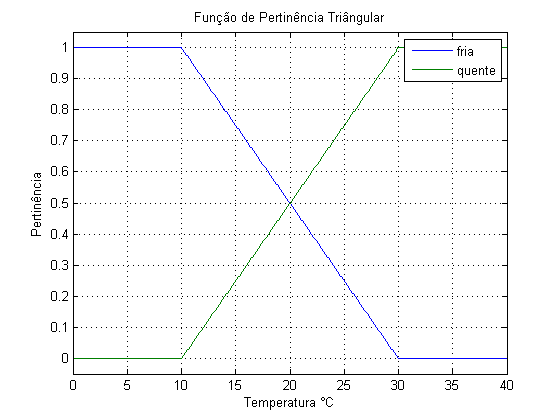
\includegraphics[width=0.5\textwidth]{img/pertinencia.png}
	\caption{Diagrama esquemático do sistema de quatro tanques e planta didática.}
	\label{figPertinencia}
\end{figure}

Nota-se que se escolhem limites para os conjuntos: toda temperatura abaixo de 10 é fria; toda temperatura acima de 30 é quente. As demais, pertencem mais ou menos à cada um dos conjuntos.

Em lógica Fuzzy, as variáveis definidas de forma subjetiva, com expressões para limites são chamadas variáveis linguísticas.




\selectlanguage{brazil}%

